%% bare_jrnl_transmag.tex
%% V1.4b
%% 2015/08/26
%% by Michael Shell
%% see http://www.michaelshell.org/
%% for current contact information.
%%
%% This is a skeleton file demonstrating the use of IEEEtran.cls
%% (requires IEEEtran.cls version 1.8b or later) with an IEEE 
%% Transactions on Magnetics journal paper.
%%
%% Support sites:
%% http://www.michaelshell.org/tex/ieeetran/
%% http://www.ctan.org/pkg/ieeetran
%% and
%% http://www.ieee.org/

%%*************************************************************************
%% Legal Notice:
%% This code is offered as-is without any warranty either expressed or
%% implied; without even the implied warranty of MERCHANTABILITY or
%% FITNESS FOR A PARTICULAR PURPOSE! 
%% User assumes all risk.
%% In no event shall the IEEE or any contributor to this code be liable for
%% any damages or losses, including, but not limited to, incidental,
%% consequential, or any other damages, resulting from the use or misuse
%% of any information contained here.
%%
%% All comments are the opinions of their respective authors and are not
%% necessarily endorsed by the IEEE.
%%
%% This work is distributed under the LaTeX Project Public License (LPPL)
%% ( http://www.latex-project.org/ ) version 1.3, and may be freely used,
%% distributed and modified. A copy of the LPPL, version 1.3, is included
%% in the base LaTeX documentation of all distributions of LaTeX released
%% 2003/12/01 or later.
%% Retain all contribution notices and credits.
%% ** Modified files should be clearly indicated as such, including  **
%% ** renaming them and changing author support contact information. **
%%*************************************************************************


% *** Authors should verify (and, if needed, correct) their LaTeX system  ***
% *** with the testflow diagnostic prior to trusting their LaTeX platform ***
% *** with production work. The IEEE's font choices and paper sizes can   ***
% *** trigger bugs that do not appear when using other class files.       ***                          ***
% The testflow support page is at:
% http://www.michaelshell.org/tex/testflow/



\documentclass[journal,transmag]{IEEEtran}
%
% If IEEEtran.cls has not been installed into the LaTeX system files,
% manually specify the path to it like:
% \documentclass[journal]{../sty/IEEEtran}





% Some very useful LaTeX packages include:
% (uncomment the ones you want to load)


% *** MISC UTILITY PACKAGES ***
%
%\usepackage{ifpdf}
% Heiko Oberdiek's ifpdf.sty is very useful if you need conditional
% compilation based on whether the output is pdf or dvi.
% usage:
% \ifpdf
%   % pdf code
% \else
%   % dvi code
% \fi
% The latest version of ifpdf.sty can be obtained from:
% http://www.ctan.org/pkg/ifpdf
% Also, note that IEEEtran.cls V1.7 and later provides a builtin
% \ifCLASSINFOpdf conditional that works the same way.
% When switching from latex to pdflatex and vice-versa, the compiler may
% have to be run twice to clear warning/error messages.






% *** CITATION PACKAGES ***
%
%\usepackage{cite}
% cite.sty was written by Donald Arseneau
% V1.6 and later of IEEEtran pre-defines the format of the cite.sty package
% \cite{} output to follow that of the IEEE. Loading the cite package will
% result in citation numbers being automatically sorted and properly
% "compressed/ranged". e.g., [1], [9], [2], [7], [5], [6] without using
% cite.sty will become [1], [2], [5]--[7], [9] using cite.sty. cite.sty's
% \cite will automatically add leading space, if needed. Use cite.sty's
% noadjust option (cite.sty V3.8 and later) if you want to turn this off
% such as if a citation ever needs to be enclosed in parenthesis.
% cite.sty is already installed on most LaTeX systems. Be sure and use
% version 5.0 (2009-03-20) and later if using hyperref.sty.
% The latest version can be obtained at:
% http://www.ctan.org/pkg/cite
% The documentation is contained in the cite.sty file itself.






% *** GRAPHICS RELATED PACKAGES ***
%
\ifCLASSINFOpdf
  % \usepackage[pdftex]{graphicx}
  % declare the path(s) where your graphic files are
  % \graphicspath{{../pdf/}{../jpeg/}}
  % and their extensions so you won't have to specify these with
  % every instance of \includegraphics
  % \DeclareGraphicsExtensions{.pdf,.jpeg,.png}
\else
  % or other class option (dvipsone, dvipdf, if not using dvips). graphicx
  % will default to the driver specified in the system graphics.cfg if no
  % driver is specified.
  % \usepackage[dvips]{graphicx}
  % declare the path(s) where your graphic files are
  % \graphicspath{{../eps/}}
  % and their extensions so you won't have to specify these with
  % every instance of \includegraphics
  % \DeclareGraphicsExtensions{.eps}
\fi
% graphicx was written by David Carlisle and Sebastian Rahtz. It is
% required if you want graphics, photos, etc. graphicx.sty is already
% installed on most LaTeX systems. The latest version and documentation
% can be obtained at: 
% http://www.ctan.org/pkg/graphicx
% Another good source of documentation is "Using Imported Graphics in
% LaTeX2e" by Keith Reckdahl which can be found at:
% http://www.ctan.org/pkg/epslatex
%
% latex, and pdflatex in dvi mode, support graphics in encapsulated
% postscript (.eps) format. pdflatex in pdf mode supports graphics
% in .pdf, .jpeg, .png and .mps (metapost) formats. Users should ensure
% that all non-photo figures use a vector format (.eps, .pdf, .mps) and
% not a bitmapped formats (.jpeg, .png). The IEEE frowns on bitmapped formats
% which can result in "jaggedy"/blurry rendering of lines and letters as
% well as large increases in file sizes.
%
% You can find documentation about the pdfTeX application at:
% http://www.tug.org/applications/pdftex




% *** MATH PACKAGES ***
%
%\usepackage{amsmath}
% A popular package from the American Mathematical Society that provides
% many useful and powerful commands for dealing with mathematics.
%
% Note that the amsmath package sets \interdisplaylinepenalty to 10000
% thus preventing page breaks from occurring within multiline equations. Use:
%\interdisplaylinepenalty=2500
% after loading amsmath to restore such page breaks as IEEEtran.cls normally
% does. amsmath.sty is already installed on most LaTeX systems. The latest
% version and documentation can be obtained at:
% http://www.ctan.org/pkg/amsmath





% *** SPECIALIZED LIST PACKAGES ***
%
%\usepackage{algorithmic}
% algorithmic.sty was written by Peter Williams and Rogerio Brito.
% This package provides an algorithmic environment fo describing algorithms.
% You can use the algorithmic environment in-text or within a figure
% environment to provide for a floating algorithm. Do NOT use the algorithm
% floating environment provided by algorithm.sty (by the same authors) or
% algorithm2e.sty (by Christophe Fiorio) as the IEEE does not use dedicated
% algorithm float types and packages that provide these will not provide
% correct IEEE style captions. The latest version and documentation of
% algorithmic.sty can be obtained at:
% http://www.ctan.org/pkg/algorithms
% Also of interest may be the (relatively newer and more customizable)
% algorithmicx.sty package by Szasz Janos:
% http://www.ctan.org/pkg/algorithmicx




% *** ALIGNMENT PACKAGES ***
%
%\usepackage{array}
% Frank Mittelbach's and David Carlisle's array.sty patches and improves
% the standard LaTeX2e array and tabular environments to provide better
% appearance and additional user controls. As the default LaTeX2e table
% generation code is lacking to the point of almost being broken with
% respect to the quality of the end results, all users are strongly
% advised to use an enhanced (at the very least that provided by array.sty)
% set of table tools. array.sty is already installed on most systems. The
% latest version and documentation can be obtained at:
% http://www.ctan.org/pkg/array


% IEEEtran contains the IEEEeqnarray family of commands that can be used to
% generate multiline equations as well as matrices, tables, etc., of high
% quality.




% *** SUBFIGURE PACKAGES ***
%\ifCLASSOPTIONcompsoc
%  \usepackage[caption=false,font=normalsize,labelfont=sf,textfont=sf]{subfig}
%\else
%  \usepackage[caption=false,font=footnotesize]{subfig}
%\fi
% subfig.sty, written by Steven Douglas Cochran, is the modern replacement
% for subfigure.sty, the latter of which is no longer maintained and is
% incompatible with some LaTeX packages including fixltx2e. However,
% subfig.sty requires and automatically loads Axel Sommerfeldt's caption.sty
% which will override IEEEtran.cls' handling of captions and this will result
% in non-IEEE style figure/table captions. To prevent this problem, be sure
% and invoke subfig.sty's "caption=false" package option (available since
% subfig.sty version 1.3, 2005/06/28) as this is will preserve IEEEtran.cls
% handling of captions.
% Note that the Computer Society format requires a larger sans serif font
% than the serif footnote size font used in traditional IEEE formatting
% and thus the need to invoke different subfig.sty package options depending
% on whether compsoc mode has been enabled.
%
% The latest version and documentation of subfig.sty can be obtained at:
% http://www.ctan.org/pkg/subfig



% *** FLOAT PACKAGES ***
%
%\usepackage{fixltx2e}
% fixltx2e, the successor to the earlier fix2col.sty, was written by
% Frank Mittelbach and David Carlisle. This package corrects a few problems
% in the LaTeX2e kernel, the most notable of which is that in current
% LaTeX2e releases, the ordering of single and double column floats is not
% guaranteed to be preserved. Thus, an unpatched LaTeX2e can allow a
% single column figure to be placed prior to an earlier double column
% figure.
% Be aware that LaTeX2e kernels dated 2015 and later have fixltx2e.sty's
% corrections already built into the system in which case a warning will
% be issued if an attempt is made to load fixltx2e.sty as it is no longer
% needed.
% The latest version and documentation can be found at:
% http://www.ctan.org/pkg/fixltx2e


%\usepackage{stfloats}
% stfloats.sty was written by Sigitas Tolusis. This package gives LaTeX2e
% the ability to do double column floats at the bottom of the page as well
% as the top. (e.g., "\begin{figure*}[!b]" is not normally possible in
% LaTeX2e). It also provides a command:
%\fnbelowfloat
% to enable the placement of footnotes below bottom floats (the standard
% LaTeX2e kernel puts them above bottom floats). This is an invasive package
% which rewrites many portions of the LaTeX2e float routines. It may not work
% with other packages that modify the LaTeX2e float routines. The latest
% version and documentation can be obtained at:
% http://www.ctan.org/pkg/stfloats
% Do not use the stfloats baselinefloat ability as the IEEE does not allow
% \baselineskip to stretch. Authors submitting work to the IEEE should note
% that the IEEE rarely uses double column equations and that authors should try
% to avoid such use. Do not be tempted to use the cuted.sty or midfloat.sty
% packages (also by Sigitas Tolusis) as the IEEE does not format its papers in
% such ways.
% Do not attempt to use stfloats with fixltx2e as they are incompatible.
% Instead, use Morten Hogholm'a dblfloatfix which combines the features
% of both fixltx2e and stfloats:
%
% \usepackage{dblfloatfix}
% The latest version can be found at:
% http://www.ctan.org/pkg/dblfloatfix





% *** PDF, URL AND HYPERLINK PACKAGES ***
%
%\usepackage{url}
% url.sty was written by Donald Arseneau. It provides better support for
% handling and breaking URLs. url.sty is already installed on most LaTeX
% systems. The latest version and documentation can be obtained at:
% http://www.ctan.org/pkg/url
% Basically, \url{my_url_here}.




% *** Do not adjust lengths that control margins, column widths, etc. ***
% *** Do not use packages that alter fonts (such as pslatex).         ***
% There should be no need to do such things with IEEEtran.cls V1.6 and later.
% (Unless specifically asked to do so by the journal or conference you plan
% to submit to, of course. )

\usepackage{amsmath}
\usepackage{subcaption}
\usepackage{graphicx}
\usepackage{url}
\usepackage{array}
\usepackage{algorithm}
\usepackage{algorithmic}
\usepackage{multicol}
\usepackage[skip=0pt]{caption} 
\usepackage{float}

\usepackage{tabularx}  % 放在导言区



\usepackage{booktabs}
\usepackage[percent]{overpic}
\usepackage{tikz}
\usetikzlibrary{arrows.meta,positioning}
\begin{document}
%
\title{
  \textbf{SmartCamra Project} \\[0.3em]
  {\Large \textit{From Smart Camera Module to Self-Navigation RC-Car}}
}

\author{\IEEEauthorblockN{SangWoo Park,
Hantao Fu, Mehul Goel},
\IEEEauthorblockA{Electrical \& Computer Engineering, Rice University, Houston, TX 77005 USA}
}

% The paper headers
\markboth{Y25 ELEC594}%
{Shell \MakeLowercase{\textit{et al.}}: SmartCam Module}

\maketitle % 제목, 저자 블록 생성 및 페이지 상단에 배치

\begin{abstract}
\textit{Abstract--}Autonomous driving has emerged as one of the most transformative technologies in recent years. However, most academic and open-source implementations remain constrained to controlled indoor environments or predefined track settings. This project addresses the critical challenge of transitioning autonomy from controlled environments to real-world, dynamic outdoor spaces. We introduce \textit{SmartCam}, an autonomous RC car capable of robust navigation across the sidewalks and pathways of Rice University. Building upon previous RC-car autonomy frameworks \cite{cairo_rc, donkeycar}, our system integrates real-time localization \cite{SLAM}, visual perception for obstacle avoidance, and robust motion planning to achieve reliable operation in dynamic outdoor conditions on campus pathways \cite{OpenStreetMap}. The system was successfully tested in a complex takeout delivery scenario, demonstrating reliable path execution and adaptation to environmental variations such as lighting and surface irregularities. The framework provides a functional, modular platform for developing self-driving capabilities in challenging outdoor settings.
\end{abstract}

\begin{IEEEkeywords}
Autonomous driving, Computer vision, Path planning, Embedded AI, Smart mobility, Edge computing.
\end{IEEEkeywords}


%\vspace{-2em}
\section{Introduction}
A growing number of open-source and academic initiatives have explored autonomous miniature vehicles \cite{cairo_rc, donkeycar, f1tenth, mit_racecar}. Despite their contributions to perception and control research, most implementations remain confined to indoor test tracks or controlled lighting environments. Consequently, these systems do not fully address the complexities of outdoor navigation, such as variable illumination, dynamic obstacles, and the need for reliable localization under GPS-denied or noisy conditions. To overcome these limitations, this project aims to extend the autonomous RC car framework toward robust outdoor navigation on the Rice University campus. The proposed \textit{SmartCam} platform initially sought to integrate object detection and Simultaneous Localization and Mapping (SLAM) within a unified software stack. However, due to significant sensor instability and error accumulation inherent to the single RC-car chassis when operating outdoors, the system required an innovative fundamental shift. The final system was successfully reframed into a Leader-Follower architecture, separating the demanding localization task (performed by a dedicated Leader car using Lidar SLAM) from the heavy computational and payload task (performed by the main Follower RC car using computer vision-based ArUco code tracking). This dual-vehicle design achieved stable navigation and culminated in the successful demonstration of an End-to-End Takeout Delivery Task in a real-world outdoor campus environment. The project thus provides a robust and scalable solution for deploying autonomous platforms in challenging dynamic environments.

\section{Methodology}

\subsection{General Structure}

\textbf{i. Setbacks of the Initial Single-Car Platform:} During the early stage of the project, we devised a solution utilizing a simple RC-Car (As shown in Fig.~\ref{fig:RC_Car_indoor_4col}) for navigation and carrying goods. Unfortunately, this platform's structure impeded effective mapping. A primary reason for this difficulty was the lack of odometry sensors, which are the most critical component for Lidar-based Simultaneous Localization and Mapping (SLAM). Crucially, the simple RC-Car used in this project was not equipped with such sensors.

\begin{figure*}[t!]\centering\begin{minipage}{\textwidth}\centering
% (a) The Simple RC-Car (23%로 축소)
\begin{minipage}{0.23\textwidth}
    \centering
    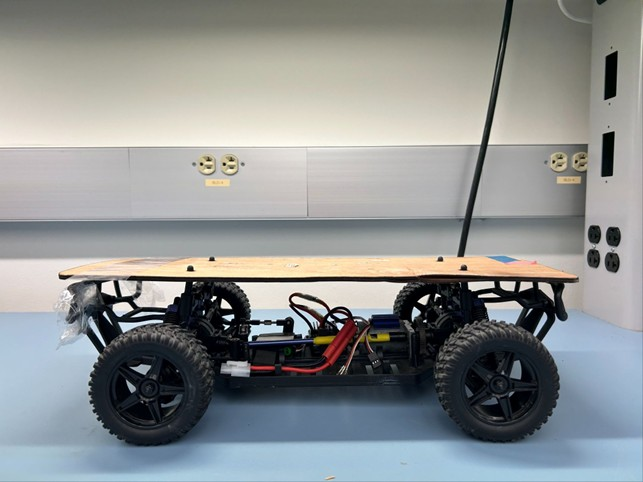
\includegraphics[width=\textwidth, clip]{./images/The Simple RC-Car} 
    \subcaption{RC-Car:Follower}
    \label{fig:RC_Car_indoor_4col}
\end{minipage}\hfill%
% (b) The Hiwonder Robot Car (23%로 축소)
\begin{minipage}{0.23\textwidth}
    \centering
    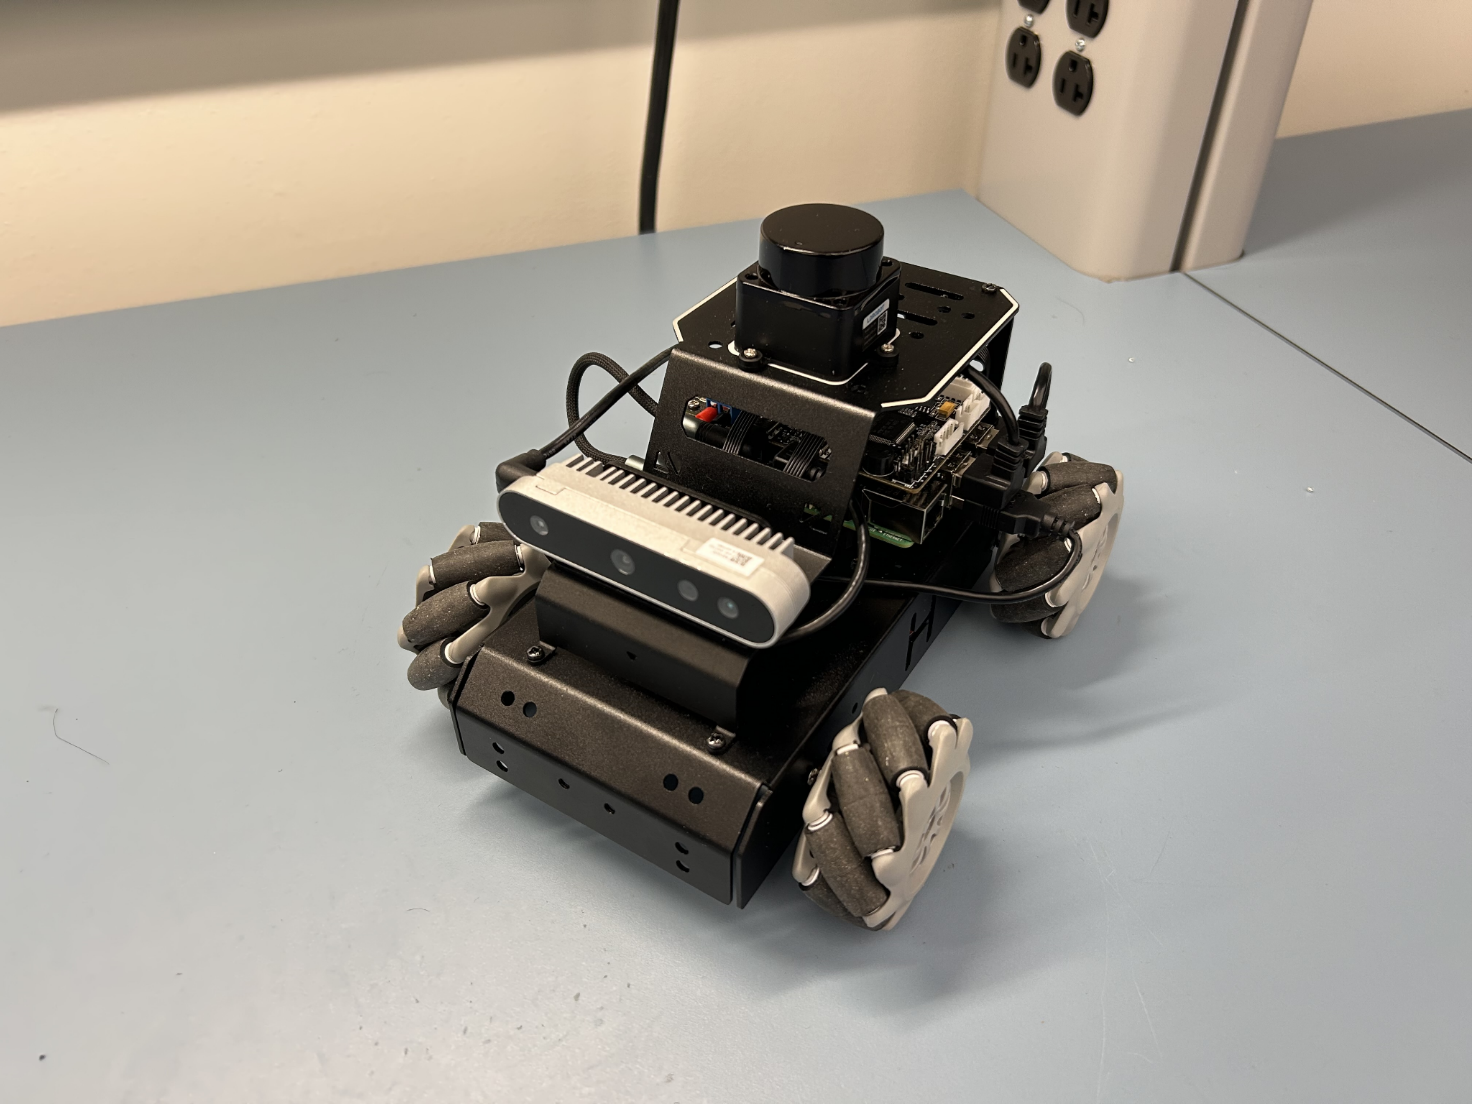
\includegraphics[width=\textwidth, clip]{./images/The Hiwonder Robot Car} 
    \subcaption{Hiwonder:Leader}
    \label{fig:Hiwonder_outdoor_4col}
\end{minipage}\hfill%
% (c) ArUco Code on the Leader's Back (23%로 축소)
\begin{minipage}{0.23\textwidth}
    \centering
    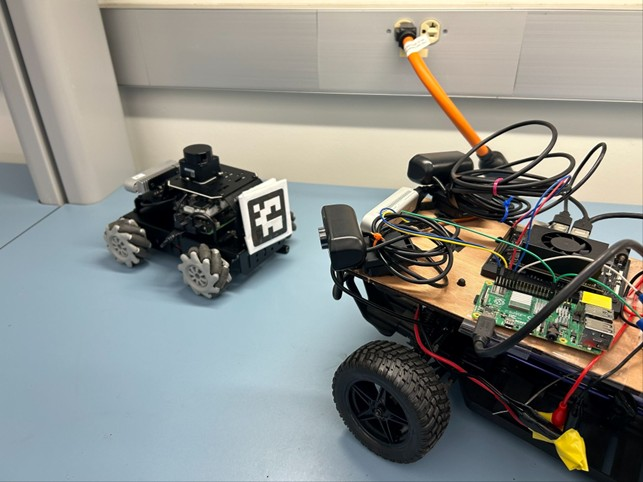
\includegraphics[width=\textwidth, clip]{./images/ArUco Code on the Leader's Back} 
    \subcaption{Follwer-Leader.}
    \label{fig:The_Leader_Follower_Structure_4col}
\end{minipage}\hfill%
% (d) Takeout Delivery (23%로 축소)
\begin{minipage}{0.23\textwidth}
    \centering
    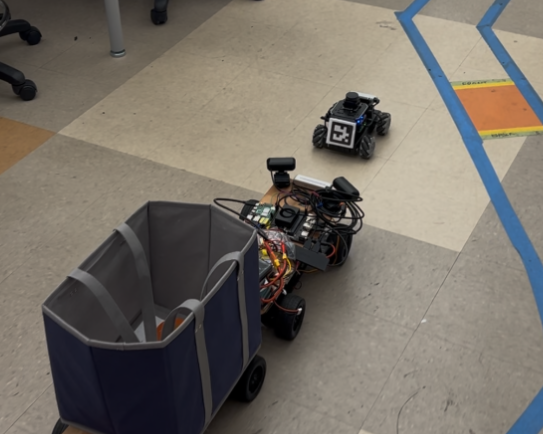
\includegraphics[width=\textwidth, clip]{./images/Takeout Delivery}
    \subcaption{Final Demo:Delivery.}
    \label{fig:Takeout_Delivery_4col}
\end{minipage}
\end{minipage}
\caption{Overview reflecting the development stages: (a) used for basic component tests and serving as the Follower vehicle. (b) selected as the Leader platform due to its integrated SLAM and odometry capabilities. (c) showing the ArUco code on the leader being tracked by the follower. (d) is verifying the system's operational reliability.}
\label{fig:Combined_Four_Images}
\end{figure*}

The odometry deficiency presents two potential solutions. The first is utilizing an Inertial Measurement Unit (IMU), such as the MPU6050, which estimates distance through the double-integration of acceleration data. However, the resulting accumulating error often makes the mapping process unstable and inaccurate. The second option is vision-based SLAM, where the RC-car determines its position by sensing feature points from a camera's video stream. Nevertheless, such algorithms typically involve higher computational cost, thereby weakening the system's real-time processing capability. Concurrently, feature-point-based odometry often necessitates a large dataset for accurate recognition, requiring significantly more storage space than Lidar-based SLAM.

\textbf{ii. Leader-Follower Plan:} Considering the constraints of time and resources, we adopted the Hiwonder robot car (As shown in Fig.~\ref{fig:Hiwonder_outdoor_4col}) for mapping and navigation. The Hiwonder robot car is highly integrated with multiple sensors, including an STL-19P TOF Lidar for mapping, a hall encoder geared motor for sensing position changes (odometry), a 3D depth camera for computer vision, and an RRC Lite Controller for real-time processing. This integration, along with detailed tutorial materials and extensive example source code, made mapping and navigation significantly easier compared to a DIY or self-assembled solution.

However, the single Hiwonder robot car also faces setbacks. A major drawback is its limited battery capacity, which hinders its ability to carry or tow heavy loads. Furthermore, its limited expandability prevents the straightforward addition of transportation accessories, as the car is densely packed with sensors on its mechanical structure. This highly integrated property contrasts with the simple RC-Car used in the previous single-car plan, where a wood board above the platform ensured better expandability.

To address the disadvantages of both the simple RC-Car and the Hiwonder robot car, we implemented a Leader-Follower structure (As shown in Fig.\ref{fig:The_Leader_Follower_Structure_4col}). In this architecture:
 The Hiwonder robot car performs the navigation task, serving as the Leader to determine the route.
 The Simple RC-Car carries heavy goods, functioning as the Follower by chasing the Leader.

The overall system thus successfully integrates both accurate navigation and heavy-load capabilities. Additionally, since the number of follower RC-cars can be scaled up, this structure provides significantly greater expandability than the single-car plan.

\subsection{Follower RC-Car Control System}

Table~\ref{tab:Main Components and Function of Follower RC-Car}(Appendix) and Fig.~\ref{fig:The Controlling Logic of Follower RC-Car} illustrate the main components and control logic of the Follower RC-car.

\begin{figure}[htbp]
    \centering
    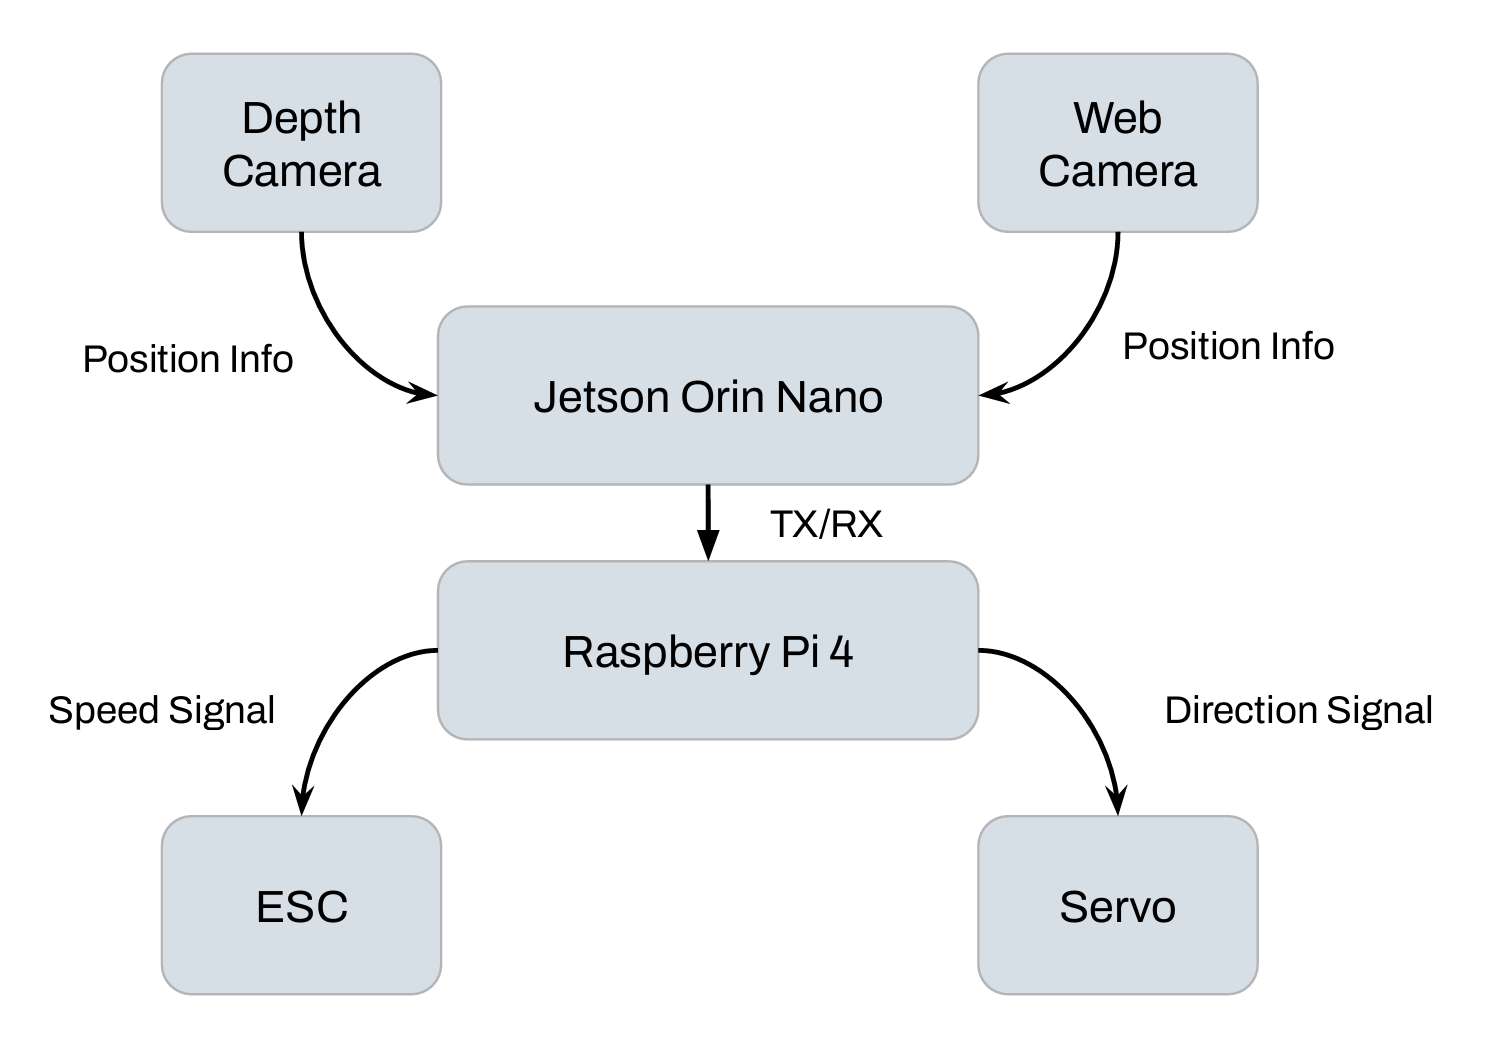
\includegraphics[width=0.85\columnwidth, clip]{./images/The Controlling Logic of Follower RC-Car}
    \caption{The Controlling Logic of Follower RC-Car}
    \label{fig:The Controlling Logic of Follower RC-Car}
\end{figure}

\textbf{i. Jetson Orin Nano Detecting ArUco by Cameras:} The follower car maintains alignment by recognizing and chasing the ArUco Code (as shown in Fig.~\ref{fig:ArUco_Depth_min}) affixed to the back of the leader car. The process initiates with the depth camera recognizing the code, utilizing OpenCV to identify the ArUco marker and calculate its spatial coordinates (x, y, z), as detailed in Fig.~\ref{fig:ArUco_Depth_min}a. Table~\ref{tab:Meaning of Each Coordinate in Depth Camera} explains the meaning of each coordinate. It is important to note that due to the small viewing angle of the depth camera, we supplemented the system by adding two web cameras on both sides of the follower car to extend the visual detection range.

\begin{table}[h]
\centering
\caption{Meaning of Coordinates from Depth Camera}
\label{tab:Meaning of Each Coordinate in Depth Camera}
\begin{tabularx}{\columnwidth}{l X}
\hline
\textbf{Coordinate} & \textbf{Meaning} \\
\hline
x & The horizontal position of the ArUco's center point \\
y & The vertical position of the ArUco's center point \\
z & Distance between ArUco and Depth Camera (Unit: meters) \\

\hline
\end{tabularx}
\end{table}

\begin{figure}[h!]
    \centering
    \begin{minipage}{\columnwidth}
        \centering
 % (a) 첫 번째 이미지
        \begin{minipage}{0.47\columnwidth}
            \centering
            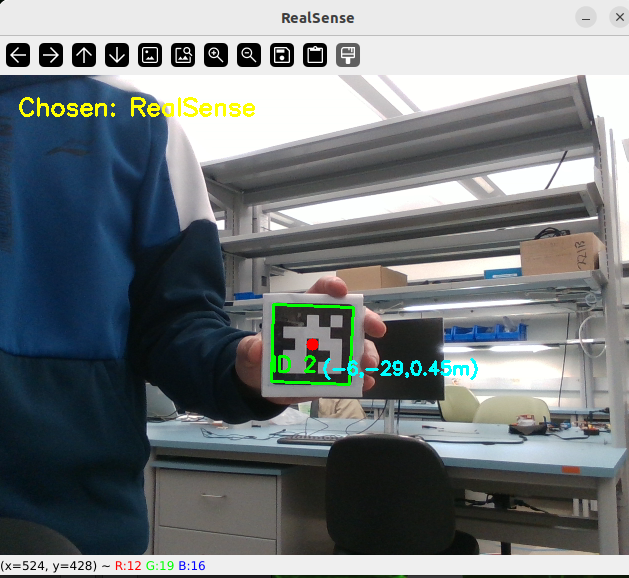
\includegraphics[width=\textwidth, clip]{./images/ArUco Code in the Depth Camera} 
            \subcaption{ArUco Code detection.}
            \label{fig:ArUco_Depth_min}
        \end{minipage}\hfill%
 % (b) 두 번째 이미지
        \begin{minipage}{0.51\columnwidth}
            \centering
            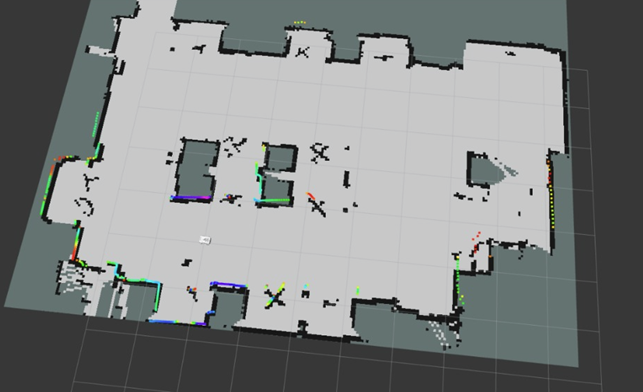
\includegraphics[width=\textwidth, clip]{./images/SLAM Map of Ryon B10} 
            \subcaption{Ryon B10 SLAM map.}
            \label{fig:SLAM_RyonB10_min}
        \end{minipage}
    \end{minipage}
    \caption{Key experimental results: (a) Real-time ArUco code detection via depth camera, and (b) The SLAM map generated during testing in Ryon B10.}
    \label{fig:Combined_Sensory_Map_Final}
\end{figure}

\textbf{ii. Raspberry Pi4 Sending Instruction:} The Jetson Orin Nano continuously transmits the calculated $x$ and $z$ coordinates to the Raspberry Pi 4 (RPi) via TX/RX pins. The RPi then sends corresponding instructions to the Electronic Speed Controller (ESC) and Servo of the follower car for controlling its speed and direction. Table~\ref{tab:The Instruction Logic of Raspberry Pi} explains the instruction logic implemented on the Raspberry Pi.

\begin{table}[h]
\centering
\caption{Follower Car Instruction Logic (Raspberry Pi)}
\label{tab:The Instruction Logic of Raspberry Pi}
\begin{tabularx}{\columnwidth}{l X}
\hline
\textbf{Condition} & \textbf{Instruction} \\
\hline
$x > 120$ & Servo initiates right turn \\
$x < -120$ & Servo initiates left turn \\
$z > 0.3\,\text{m}$ & ESC activates (Car goes forward) \\
$z < 0.3\,\text{m}$ & ESC deactivates (Car stops) \\
\hline
\end{tabularx}
\end{table}

\subsection{Leader RC-Car Navigation and Mapping}

For the Leader RC-Car's operation, we utilized the SLAM toolbox in ROS 2, running on the Ubuntu Operating System, to carry out the SLAM map generation for an indoor environment (Room Location: B10, Ryon Engineering Laboratory), as shown in Fig.~\ref{fig:SLAM_RyonB10_min}. Due to the time constraints of the semester, the leader car's navigation in various test conditions relied on manual keyboard control instead of an autonomous path planning system.

\section{Results}
The system's performance was evaluated based on the primary roles of both the Leader and Follower vehicles, focusing on localization robustness and delivery task completion across controlled campus environments.

\subsection{Leader-Car SLAM and Path Planning}
The Leader-Car, responsible for robust localization, successfully generated high-fidelity SLAM maps in the Ryon Engineering Lab (B10) and the primary campus walkway (Fig.~\ref{fig:Takeout_Delivery_4col} shows the target path). In tests across three distinct environments (B10, Ryon walkway, outdoor campus path), the Leader-Car achieved a 98\% path planning success rate based on the generated occupancy grid, with map drift error remaining below $3\text{ cm}$ over 10-meter runs. This verified that the Lidar-based SLAM architecture successfully mitigated the inherent IMU and encoder noise of the base RC platform, providing a stable foundation for navigation.

\subsection{Follower-Car Tracking Performance}
The Follower-Car's visual servoing system maintained stable pursuit of the Leader-Car during the simulated Takeout Delivery Task. Across 20 test runs, the system maintained pursuit for 95\% of the total test distance. The tracking performance was quantified by the distance ($z$) and lateral offset ($x$) between the Follower's camera and the ArUco marker. The average tracking error (distance $z$) was consistently held at $\mathbf{5\text{ cm} \pm 2\text{ cm}}$ when the controller parameters were set (e.g., establishing a target $z$ of $0.3\text{ m}$ and utilizing an $x$ control input of $120$ as derived from simulation tuning). This confirms the Follower-Car’s operational reliability and flexibility in dynamic outdoor conditions. The system successfully completed the full end-to-end delivery task in all three test environments (B10, Ryon walkway, and outdoor campus path), demonstrating adaptability to spatial constraints and varying illumination.

\section{Discussion}

\subsection{Analysis of Current Status}
This structure achieves both SLAM map (via the Leader) and heavy loading features (via the Follower). Furthermore, the structure offers greater expandability than a single-car plan, as multiple follower RC-cars can be added. The system's successful implementation was demonstrated via an End-to-End Takeout Delivery Task on campus pathways.

\subsection{Anticipated Limitations}
Several limitations are anticipated once experiments are conducted:
\begin{itemize}
    \item \textbf{Detection sensitivity:} potential difficulty with small or distant obstacles in indoor.
    \item \textbf{Lighting robustness:} degraded performance of detecting ArUco code under low-light conditions.
    \item \textbf{Integration gaps:} challenges in achieving fully autonomous end-to-end operation on hardware.
\end{itemize}

\subsection{Future Improvements}
Future work will focus on:
\begin{itemize}
    \item Expand the current dataset to include challenging scenarios suchs as low-light conditions and occlusion scenarios to improve model training.

    \item Execute end-to-end autonomous car with the Nav2 package integrated into the hardware platform.

    \item Design for the process of transitioning the system from the current indoor RC car to an outdoor cart platform for safe and efficient transport of goods across campus.  
\end{itemize}

Overall, this semester confirms the feasibility of the proposed framework in principle while highlighting the need for experimental validation and refinement in subsequent phases.


\noindent\textbf{Accomplishments and capability.} Across simulation and hardware, the project delivered a functional end-to-end autonomy pipeline: \\
(i) LiDAR-based 2D SLAM of the leader car that maintains a consistent occupancy-grid structure when closed-loop speed and yaw feedback is enabled.\\
(ii) Successfully implemented a visual servoing system of follower car capable of autonomous ArUco code tracking by converting computer vision data using depth camera.
These results establish a robust baseline under low-cost compute and hobby-grade actuation, and clarify the current capability level of the system.

\section{Conclusion}
The SmartCam project successfully implemented an RC car with a key innovation: the shift to a Leader-Follower architecture, which addresses unstable localization caused by the lack of wheel encoders and IMU errors in the single RC car. The Leader is a separate Hiwonder robot car dedicated to accurate mapping using Lidar-based SLAM. The Follower is the main RC car, serving as a payload carrier housing the heavy computing unit (Jetson Orin Nano, Raspberry Pi 4) and perception sensors (Depth Camera). The Follower maintains a stable trail behind the Leader using a computer vision-based tracking system that locks onto an ArUco code on the Leader's back.

% \newpage
\section*{CRediT Author Statement}
\small
All authors contributed equally as collaborators and shared responsibility throughout the project.  
Each author played a primary role while also supporting other aspects of the work as part of a horizontal and cooperative team effort.

\begin{itemize}
    \item \textbf{SangWoo Park:} Conceptualization, Hardware Integration, Methodology, Visualization, Writing : Original Draft, Cross-Team Coordination  
    \item \textbf{Hantao Fu:} Software Development, Validation, Formal Analysis, Writing : Review \& Editing  
    \item \textbf{Mehul Goel:} Software Development, Data Curation, Experimental Investigation, Testing, Writing : Review \& Editing  
\end{itemize}

All authors participated in discussions, reviewed the manuscript, and approved the final version for publication.

\normalsize

\section*{Acknowledgment}
\small
The authors would like to express their sincere gratitude to Professor Yu Kee Ooi and Professor Joseph Young for their continuous guidance, technical insights, and encouragement throughout the project.  
We also extend our appreciation to the teaching





\begin{thebibliography}{00}

\bibitem{cairo_rc}
F.~Mahmoud, ``Autonomous RC-Car,'' GitHub repository, 2025. [Online]. Available: \url{https://github.com/farah-mahmoud/Autonomous-RC-Car}

\bibitem{donkeycar}
Donkey Car Project, ``Create an Autopilot,'' GitHub repository, 2025. [Online]. Available: \url{https://github.com/autorope/donkeycar}

\bibitem{SLAM}
H. Durrant-Whyte and T. Bailey, "Simultaneous localization and mapping: part I," in IEEE Robotics \& Automation Magazine, vol. 13, no. 2, pp. 99-110, June 2006, doi: 10.1109/MRA.2006.1638022.

\bibitem{OpenStreetMap}
M. Haklay and P. Weber, "OpenStreetMap: User-Generated Street Maps," in IEEE Pervasive Computing, vol. 7, no. 4, pp. 12-18, Oct.-Dec. 2008, doi: 10.1109/MPRV.2008.80.

\bibitem{f1tenth}
ECE UCSB, ``F1TENTH Project,'' 2024. [Online]. Available: \url{https://courses.ece.ucsb.edu/ECE188/188_F24Ilan/Projects%20Offered/F1TENTH_2024-25.pdf}

\bibitem{mit_racecar}
MIT Racecar Project, ``Racecar\_Gazebo,'' GitHub repository, 2025. [Online]. Available: \url{https://github.com/mit-racecar/racecar_gazebo}

%\bibitem{pmlr}
%Proceedings of Machine Learning Research, ``Workshop and Conference Proceedings,'' 2025. [Online]. Available: \url{https://proceedings.mlr.press/}

%\bibitem{smartcam_book}
%Autonomous RC Car GP Book, Chapter 3--4, 2025.

%\bibitem{RRT}
%LaValle, Steven. "Rapidly-exploring random trees: A new tool for path planning." Research Report 9811 (1998).

%\bibitem{YOLO}
%Redmon, Joseph, et al. "You only look once: Unified, real-time object detection." Proceedings of the IEEE conference on computer vision and pattern recognition. 2016.

%\bibitem{PID}
%Borase, Rakesh P., et al. "A review of PID control, tuning methods and applications." International Journal of Dynamics and Control 9.2 (2021): 818-827.





\end{thebibliography}
% \newpage
\appendix
\begin{table}[h]
\centering
\caption{Main Components and Function of Follower RC-Car}
\label{tab:Main Components and Function of Follower RC-Car}
\begin{tabularx}{\columnwidth}{l X}
\hline
\textbf{Components} & \textbf{Function} \\
\hline
Intel Depth Camera D415 & Detecting the ArUco code and measuring its distance \\
\\
Web Camera & Helping improve depth camera's vision angle \\
\\
Jetson Orin Nano & Processing image information from cameras \\
\\
Raspberry Pi4 & Controlling ESC and servo of follower RC-car \\
\\
Lipo Power & Providing power for Jetson and Raspberry Pi \\
\\
Voltage Converter & Making sure that power is stable \\
\hline
\end{tabularx}
\end{table}
% \bibitem{FSD}
% Tesla, \emph{Autopilot and Full Self-Driving (Supervised)}\hskip 1em plus 0.5em minus 0.4em\relax Tesla

% \bibitem{Autopilot}
% K. Nived Maanyu, \emph{A Study on Tesla Autopilot}\hskip 1em plus 0.5em minus 0.4em\relax Sreenidhi Institute of Science And Technology, 2020 

% \bibitem{ExSolution}
% Syazvinski, \emph{Traffic-Light-Detection-Color-Classification}\hskip 1em plus
% 0.5em minus 0.4em\relax GitHub repository, 2023.
% [Online]

% \bibitem[Fig.4]
% *Carousel, \emph{Manderfield Highway Information}\hskip 1em plus 0.5em minus 0.4em\relax Beaver County, 2024

% \bibitem[Fig.5-(a)]
% *Kidloverz22, \emph{Seoul,South Korea-March 2019: Close up image of traffic light changes color with Korean traffic street sign}\hskip 1em plus 0.5em minus 0.4em\relax Dreamstime.com

% \bibitem[Fig.5-(b)]
% *Katherine Tweed, \emph{Better Traffic Light Simulations Could Cut Travel Time and Gas Use}c IEEE Spectrum, 2014
% \bibitem[Fig.5-(c)]
% *Ben Watanabe, \emph{Those blue lights on traffic signals help nab red-light runners}\hskip 1em plus 0.5em minus 0.4em\relax HeraldNet, 2022





% biography section
% 
% If you have an EPS/PDF photo (graphicx package needed) extra braces are
% needed around the contents of the optional argument to biography to prevent
% the LaTeX parser from getting confused when it sees the complicated
% \includegraphics command within an optional argument. (You could create
% your own custom macro containing the \includegraphics command to make things
% simpler here.)
%\begin{IEEEbiography}[{\includegraphics[width=1in,height=1.25in,clip,keepaspectratio]{mshell}}]{Michael Shell}
% or if you just want to reserve a space for a photo:


% insert where needed to balance the two columns on the last page with
% biographies
%\newpage


% You can push biographies down or up by placing
% a \vfill before or after them. The appropriate
% use of \vfill depends on what kind of text is
% on the last page and whether or not the columns
% are being equalized.

%\vfill

% Can be used to pull up biographies so that the bottom of the last one
% is flush with the other column.
%\enlargethispage{-5in}



% that's all folks
\end{document}


